\documentclass{article}
\usepackage[UTF8]{ctex}
\usepackage{geometry}
\usepackage{multirow}
\usepackage{natbib}
\geometry{left=3.18cm,right=3.18cm,top=2.54cm,bottom=2.54cm}
\usepackage{graphicx}
\pagestyle{plain}
\usepackage{setspace}
\usepackage{enumerate}
\usepackage{caption2}
\usepackage{datetime} %日期
\renewcommand{\today}{\number\year 年 \number\month 月 \number\day 日}
\renewcommand{\captionlabelfont}{\small}
\renewcommand{\captionfont}{\small}
\begin{document}

\begin{figure}
    \centering
    
\includegraphics[width=8cm]{upc.png}

    \label{figupc}
\end{figure}

	\begin{center}
		\quad \\
		\quad \\
		\heiti \fontsize{45}{17} \quad \quad \quad
		\vskip 1.5cm
		\heiti \zihao{2} 《计算科学导论》个人职业规划
	\end{center}
	\vskip 2.0cm

	\begin{quotation}
% 	\begin{center}
		\doublespacing

        \zihao{4}\par\setlength\parindent{7em}
		\quad

		学生姓名:\underline{\qquad  田康康 \qquad \qquad}

		学\hspace{0.61cm} 号:\underline{\qquad 1606050112\qquad}

		专业班级:\underline{\qquad 计科1702 \qquad  }

        学\hspace{0.61cm} 院:\underline{计算机科学与技术学院}
% 	\end{center}
		\vskip 1.5cm
		\centering
		\begin{table}[h]
            \centering
            \zihao{4}
            \begin{tabular}{|c|c|c|c|c|c|c|c|c|}
            % 这里的rl 与表格对应可以看到,姓名是r,右对齐的;学号是l,左对齐的;若想居中,使用c关键字。
                \hline
                \multicolumn{5}{|c|}{分项评价} &\multicolumn{2}{c|}{整体评价}  & 总    分 & 评 阅 教 师\\
                \hline
                自我 & 环境 & 职业 & 实施 & 评估与 & 完整性 & 可行性 &\multirow{2}*{} &\multirow{2}*{}\\
                分析& 分析& 定位 & 方案 & 调整 & 20\% & 20\% & ~&~ \\\
                10\% & 10\% & 15\% & 15\% & 10\% & &  &~ &~\\
                \cline{1-7}
                & & & & & & & ~&~ \\
                & & & & & & & ~&~ \\
                \hline
            \end{tabular}
        \end{table}
		\vskip 2cm
		\today
	\end{quotation}

\thispagestyle{empty}
\newpage
\setcounter{page}{1}
% 在这之前是封面,在这之后是正文
\section{自我分析}
	% 自我分析即对自己进行全方位、多角度的分析,目的是认识自己、了解自己。只有认识了自己,才能对自己的职业做出正确的选择,才能选定适合自己发展的职业生涯路线,才能对自己的职业生涯目标做出最佳抉择。\par
	% 自我分析包括:\par
\subsection{自然条件}
% 性别、年龄、身体条件、健康状况、居住城市等。\par
性别男,年龄22岁,身体条件还可以,偏瘦,计划在大四学年增重、运动。家庭住址济南市商河县,山东省经济倒数的县城,发展极差。
\subsection{性格分析}
我自认为性格比较平和冷淡,从初中便开始宿舍住宿生活,对各种人性有极强的适应能力,轻易不会被触及底线。对待熟悉的人非常热情,与性格合得来的人关系发展很快。
\subsection{教育与学习经历}
小学在乡镇小学读书,然后初中高中均在县排名第一的中学,现在大部分保持联系的朋友都是高中同学,初中小学的经历对我的影响很小。
\subsection{工作与社会阅历}
工作与社会阅历基本为0,会在大四暑假去参加实习,增加自己的工作经验。当然如果算上在社交媒体、网络资讯上了解的社会现状的话,我觉得大部分都是负能量的,我并没有被它们所影响,希望真实的社会可以给我洗礼。
\subsection{知识、技能与经验}
这方面除了在学校里学习到的,我大部分的知识都与计算机有关,相比于其他,我更喜欢敲击键盘的快乐,掌握最新的技术。
\subsection{兴趣爱好与特长}
兴趣爱好就是新事物,学习新的框架,新的架构,发掘互联网上的秘密,发现最新奇的应用,喜欢一切科技相关。我的特长也是在我的兴趣爱好发展中建立起来的,我擅长利用互联网找到我想要的资源、需要的信息。
\section{环境分析}
我从小生活在济南,大学在青岛呆了四年了(转专业降级一级),这两个地方简直就是IT荒漠,往更大的范围来说,整个山东都是IT荒漠。我从小学开始熟悉计算机,而直到我上了大学,都没有找到几个可以和我有关于计算机方面的共同语言的人,我以为我转专业之后
在计算机科学与技术专业可以有这种人,但还是没有几个。这已经不是地区的问题了,我以后工作的话一定会去极客氛围浓厚的地区,恋爱也要与对计算机对新事物感兴趣的人恋爱。我真的难以想象作为前沿学科的学生,就只会课堂上老师教的知识,对新事物没有追求,
甚至到了大三了还只会写单文件项目,没听说过Javascript更别说Typescript。呆在这种环境里,可怕。
\subsection{社会环境分析}
今年的经济形势其实挺差的,互联网寒冬,还恰逢中美贸易战,无数公司大范围裁员,甚至国务院都印发了《关于进一步做好稳就业工作的意见》,提到了“防范化解规模性失业风险”,工作太难了。政治形势也非常严峻,中美贸易战不只是贸易战,还是政治战。总之,
各方面的形式都非常严峻,没有实力难以突围。
\subsection{家庭环境分析}
% 婚姻状况、经济状况、家人期望、家族传统等。\par
家庭环境没有太多可以分析的,只是普通家庭的一户,我的父母也支持我去大城市,去奋斗。
\subsection{职业环境分析}
% 行业现状及发展趋势;职业的工作内容、工作要求、发展前景等。\par
我的意向工作方向是全栈或者前端,首选是前端,前端在北上广的薪资普遍在13K-20K之间,岗位还是挺多的。但是现在前端的工作已经不是以前那种写几个页面就能解决的了,现在发展比较科学的几个公司都是“大前端”的架构方式,前端已经不止需要会CSS、HTML、JS,
还需要掌握主要的框架、设计模式,甚至需要有一定的服务端编程能力。对真正有能力的前端的需求只会越来越多,薪资也会越来越高。
\begin{figure}[h!]
\centering
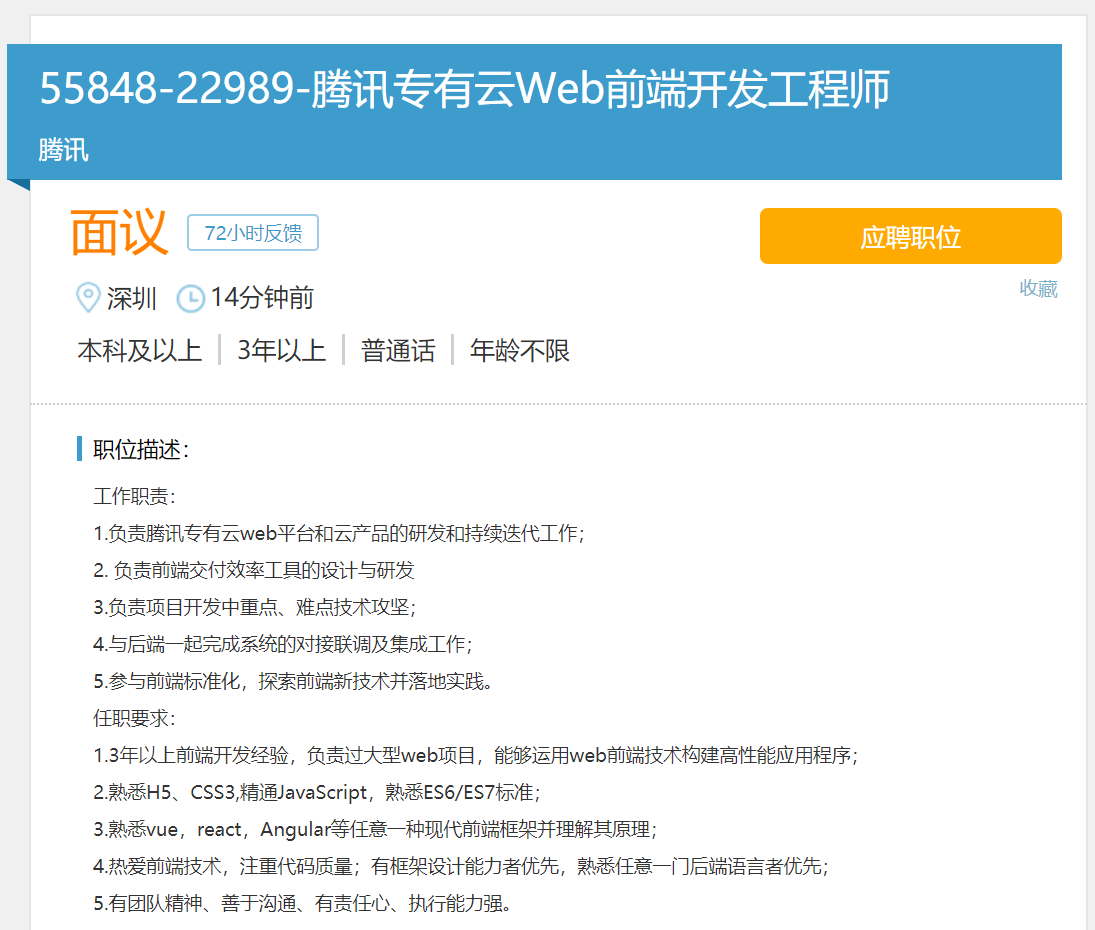
\includegraphics[scale=0.2]{gongzuo.png}
\caption{腾讯的前端工程师要求}
\label{fig:job}
\end{figure}

\subsection{地域与人际环境分析}
% 工作城市的气候水土、文化特点、发展前景;人脉与人际关系等。\par
我的意向工作城市是成都或者南京,如果单纯为了工作的话我会选择深圳。选择成都或者南京的原因其实是美食比较多,环境也比北方的城市好一些,因为这些原因我可以放弃一部分薪资选择这两个城市。单纯为了工作为了赚钱的话我会选择深圳,深圳的工作机会真的太多了,
而且平均薪资也远高于上述城市,也是在南方,环境好,深圳一直在发展,未来也会发展的更好,选择深圳不用考虑城市的发展问题。人脉与人际关系在上述城市都基本为0,选择去这些城市都需要一切从头开始,一个人面对社会的洗礼,作为北方人,各方面习惯与南方人也天差地别,
我只能说,让暴风雨来的更猛烈些吧!
% \par
% 图片插入的样例:\par
% \begin{figure}[h!]
% \centering
% \includegraphics[scale=1.7]{universe}
% \caption{The Universe}
% \label{fig:universe}
% \end{figure}

\section{职业定位}
% 在准确地对自己和环境做出了分析之后,确定适合自己行业和有实现可能的职业发展目标。职业定位时要注意与自己的自然条件、知识背景、技能特长、性格特点、兴趣爱好是否匹配,考虑与自己所处的环境是否相适应。职业定位决定了职业发展中的行为和结果,是制定职业生涯规划的关键,应当科学合理,具有可行性。\par
% 职业定位包括:\par

\subsection{行业领域定位与理由}
行业领域:程序员。\par
理由:相对于做理论研究,我更喜欢看到我脑海中构思的事物通过代码构造出来,有代码就够了。

\subsection{职业岗位起点定位与理由}
岗位起点:前端工程师\par
相对于后端程序员、算法工程师等岗位,前端工程师做到即写即现是成本最低的,而且现在有了Node.JS,我可以更简单的实现全栈编程,向全栈工程师前进。
\subsection{职业目标与可行性分析}
% 成果目标、经济目标、能力目标、职务目标等。\par
\begin{enumerate}[(1)]
	\item 短期目标(大学4年)\par
	我的大学基本过完了,我现在的短期目标就是前段水平达到大厂对前端应届生的要求,进大厂。
	\item 中长期目标(5-10年)\par
	成为全栈工程师。毕业五-八年内攒够首付,争取在南京或者成都定居,实现电子产品自由,即最新的电子产品可以不考虑价格直接购买体验。独立开发一个前端UI框架,类似Layui。
\end{enumerate}
% 这里是简单列表的样例:(如果需要标号自定义或者自动标记数字序号,请自行搜索语法)
% \begin{itemize}
%     \item 简单的列表结构
%     \item 如这里所示
%     \item 此处仅为样例
%     \item 按需修改和使用
% \end{itemize}


\section{实施方案}
% 在明确了职业定位后,要制定实现职业生涯目标的行动方案,不付诸行动,职业目标只能是一种梦想。实施方案是实现职业目标的保证,尽量考虑周全、具有可操作性。\par
% 实施方案可以从以下角度考虑:\par
\begin{enumerate}[1、]
	\item 如何利用现有条件和自身优势以实现职业生涯目标。\par
	作为普通大学生一名,现有的大部分条件相对于其他同学来说并没有优势,甚至更差。相对于同学们的优势应该只有项目经验的优势,我在学习之余写过一些练手的项目,有全栈、爬虫、JS等项目,争取把这个优势扩大。
	\item 如何克服缺点、弥补不足、增长知识、提高能力以实现职业生涯目标。\par
	我计划在大三下学期与大四上学期完成一个大的前端项目,具体的项目架构还没有确定,我希望能通过自己独立地创造性地完成一些项目来提高自己的竞争力,相信完成这样一个项目可以让我对编程语言、算法等有更深刻的认识,
	帮助我实现自己的短期目标。
	\item 如何处理人际关系和发展人脉以实现职业生涯目标。\par
	首先要与同学们处理好关系,毕竟大学同学长期来看是涉及最广泛的人脉关系。对于不准备考研的我来说,还需要考虑的是当外出参加实习、找工作的时候,与周围的同事处好关系,与历届校友学长取得联系,争取获得大厂的内推名额或者及时获取大厂的招聘信息。
	\item 如何处理工作与家庭、生活的关系以实现职业生涯目标。\par
	在短期内,为了提升自己的价值,需要在工作之余尽可能提高自己的技术修养,提高自己的能力,不能成为只会工作的机器,待干不动了之后便被抛弃。当然,有一个温馨的家也很重要,如果只有自己一个人,天天工作学习形单影只,可能很快就崩溃了,
	但是为了未来肯定难以协调好工作与家庭之间的关系,现在的我没有办法做出规划,为了未来,我可能会放弃一部分当下。
	\item 如何处理释放工作压力、保证身心健康以实现职业生涯目标。\par
	发展一些业余的爱好,尽量保持规律的运动,固定时间健身、骑行。既是防止猝死,也是为了让自己能保持活力,毕竟有活力有动力才能好好工作。
\end{enumerate}
\par
% 表格插入样例(三线表):\par
% %单元格怎么写?参考第一页打分的表格

% \begin{table}[h]
% 	\centering
% 	\caption{这是科学系的花名册}
% 	\begin{tabular}{rl}
% 		% 这里的rl 与表格对应可以看到,姓名是r,右对齐的;学号是l,左对齐的;若想居中,使用c关键字。
% 		\hline
% 		姓名 & 学号 \\
% 		\hline
% 		张三 & 190704xxxx+++ \\
% 		李四 & 190704yyyy \\
% 		王二五 & 190704zzzz\\
% 		\hline
% 	\end{tabular}
% 	\label{table1}
% \end{table}
\section{评估与调整}
% 由于影响职业生涯规划的因素很多,且大都处于动态变化之中,因此职业生涯规划应定期评估,并根据影响因素的变化和实施结果的情况及时作出调整,这样才能保证其行之有效。\par
现在各种新技术层出不穷,各种新的框架、新的思想都在迸发。就近几年,前端已经从只需要搭积木变成了对算法、浏览器底层要熟悉,现在又有了“大前端”的雏形,各种工作岗位在不断的细分与融合,很难想象在未来五年、十年,
现在热门的概念、框架会发展成什么样子。还有当今的政治形势与经济形势也是飞速变化,可能今天明天就天翻地覆,很难掌控。所以要在尽可能短的时间周期中进行评估与调整,及时作出改变,调整计划。
\subsection{评估时间}
% 可以选择每学期评估一次、每学年一次、三年评估一次。\par
一年评估一次,如果有重大政治、经济事件则即时评估。
\subsection{评估内容}
% 可以从成果目标、经济目标、能力目标、职务目标等方面总结,确定哪些目标已按预期实现,哪些目标商未达到,对已实现的成果总结经验,对未完成的目标分析原因。\par
我更倾向于评估自己当时的短期目标与长期目标和当时的技术趋势、政治经济情况之间的关系。长远来看,技术趋势、政治经济趋势都会对行业发展造成巨大影响。
\subsection{调整原则}
% 应考虑与自身情况的匹配性、与环境的适应性、操作实施的可行性等。\par
以自身发展为主,尽量在不影响其他人的情况下做出调整。当然,以后踏上社会之后为了生活可能有很多事情是身不由己的,这种事情无法提前判断和规避,只能随机应变,这里就不赘述。




\end{document}
